\documentclass[journal]{vgtc} 
\usepackage{hs-vis_ss10}


%% Please note that the use of figures other than the optional teaser
%% is not permitted on the first page of the journal version.  Figures
%% should begin on the second page and be in CMYK or Grey scale
%% format, otherwise, colour shifting may occur during the printing
%% process.  Papers submitted with figures other than the optional
%% teaser on the first page will be refused.

%% These three lines bring in essential packages: ``mathptmx'' for
%% Type 1 typefaces, ``graphicx'' for inclusion of EPS figures. and
%% ``times'' for proper handling of the times font family.

\usepackage{mathptmx} 
\usepackage{graphicx}
\usepackage{times}
\usepackage{amsmath}
\usepackage{amssymb}

%% allow for this line if you want the electronic option to work
%% properly
\vgtcinsertpkg


%% author name
\author{Moritz Hamann}

%% paper title
\title{Clustering of dynamic graphs}

%% short title for header
\shorttitle{Clustering of dynamic graphs}


%% Abstract section.
\abstract{%
Betrachtet man die Graphen realer Netzwerke stellt man fest, dass die Kantenverteilung lokal oftmals stark variiert. In solchen Graphen
sind vor allem diejenigen Teilgraphen von Interesse, welche eine hohe Kantendichte haben und deren Knoten stark verkn"upft sind.
Diese Teilgraphen werden auch Cluster genannt.

In diesem Artikel wird eine Zusammenfassung verschiedener Verfahren gegeben, welche solche Cluster in einem Graph finden. Neben dem
Clustering klassischer statischer Graphen, werden auch Verfahren vorgestellt, die auf zeitver"anderlichen dynamischen Graphen operieren.
Hierzu wird im ersten Teil eine kurze Einf"uhrung in die wichtigsten Eigenschaften von Cluster, k-Cliques und dynamischen Graphen gegeben.

Anschlie"send wird eine "Ubersicht verschiedener Clusteringverfahren f"ur statische Graphen pr"asentiert, ihre grundlegenden Funktionsweisen
erl"autert und anhand dieser eine Einteilung in verschiedene Klassen vorgenommen. Hierbei werden exemplarische die Modularit"atsoptimierung,
sowie die Clique Percolation Method als zwei Vertreter dieser Algorithmen genauer erl"autert.

Im letzten Teil werden zwei Verfahren vorgestellt, mit denen Cluster auch in dynamischen Graphen gefunden werden k"onnen. Neben einer
Erweiterung der Clique Percolation Method, wird ein sogenanntes Time-Step Clustering pr"asentiert, welches erm"oglicht beliebige
statische Clusteringverfahren auch auf dynamische Graphen anzuwenden.
} % end of abstract


%% Uncomment below to include a (optional) teaser figure.
\teaser{ \centering
  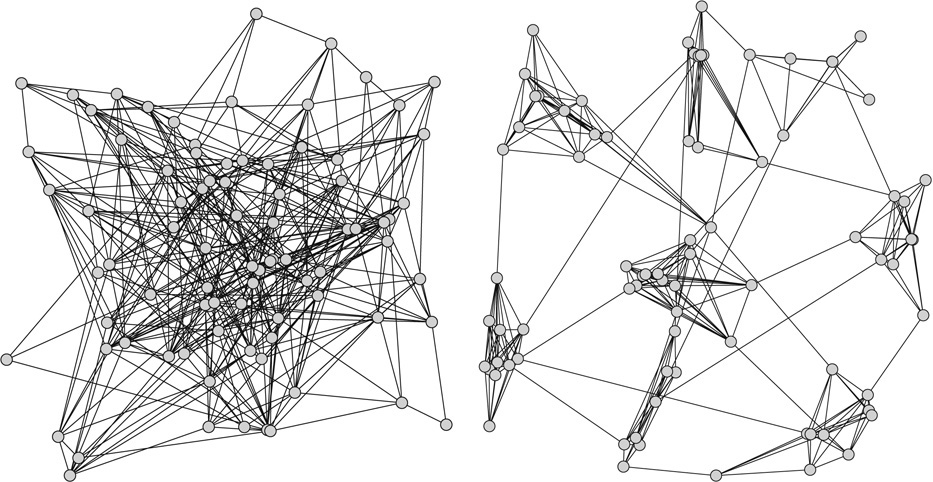
\includegraphics[width=16cm]{images/teaser}
  \caption{Zwei Graphen mit je 84 Knoten und 358 Kanten, welche beide mit einem Spring-Force Algorithmus visualisiert wurden. Man sieht deutlich die
  lokalen Inhomogenit"aten im linken Graph, der eine ``Relaxed Caveman'' Struktur hat. Der rechte Graph ist ein  zuf"alliger Random Graph \cite{Schaeffer}}
}


%%%%%%%%%%%%%%%%%%%%%%%%%%%%%%%%%%%%%%%%%%%%%%%%%%%%%%%%%%%%%%%%
%%%%%%%%%%%%%%%%%%%%%% START OF THE PAPER %%%%%%%%%%%%%%%%%%%%%%
%%%%%%%%%%%%%%%%%%%%%%%%%%%%%%%%%%%%%%%%%%%%%%%%%%%%%%%%%%%%%%%%%

\begin{document}

%% The ``\maketitle'' command must be the first command after the
%% ``\begin{document}'' command. It prepares and prints the title
%%   block.

%%   the only exception to this rule is the \firstsection command
\firstsection{Motivation}
\maketitle

  Das mathematische Konzept der Graphen ist ein essentielles 
  Modellierungswerkzeug in der Informatik. Nicht nur lassen sich damit
  verschiedenste Datenstrukturen anschaulich dargestellten, sondern
  mit ihrer Hilfe lassen sich auch jegliche Beziehungen zwischen einzelnen
  Objekten oder Prozessen in einem Netzwerk modellieren und untersuchen.
  Aus diesem Grund sind sie heutzutage nicht nur in der klassischen Informatik
  sowie in der Mathematik zu finden, sondern haben auch in vielen anderen
  Wissenschaften ihren Einzug erhalten. So werden sie genutzt um die
  Gruppendynamik in biologischen Netzwerken zu beschreiben, dienen
  als Kontrollalgorithmen für Multiagenten Systeme \cite{graphcontrol} und beschreiben
  Kommunikationsmuster in sozialen Netzwerken.
  
  Um die Eigenschaften sehr großer Netzwerke analytisch untersuchen zu können,
  werden häufig Zufallsgraphen nach dem Model von Edgar Gilbert (nachweise?) oder
  Erdos-Renyi verwendet. Diese Graphen haben die Besonderheit, dass die 
  Wahrscheinlichkeit für eine Verbindung zwischen je zwei Knoten im 
  gesamten Netzwerk konstant ist. Dadurch entsteht ein gleichmäßiger Graph,
  dessen Gradverteilung binomial verteilt sind, und somit die meisten Knoten 
  die gleiche Anzahl an Kanten haben. Mit Hilfe der Wahrscheinlichkeitstheorie,
  lassen sich nun die Eigenschaften dieser Graphen auch für eine sehr hohe Anzahl
  an Knoten bestimmen und untersuchen.
  
  Allerdings haben Untersuchungen von realen Netzen gezeigt (Nachweis), dass sich
  diese in den meisten Fällen von Zufallsgraphen unterscheiden. Reale Netzwerke sind
  häufig sogenannte Skalen freie Netze (im Englischen 'Scale-free networks'), in 
  denen die Anzahl der Verbindungen pro Knoten nicht binomial verteilt ist, sonder nach einem
  Potenzgesetz. Dadurch einsteht ein Netzwerk, in dem einzelne wenige Knoten eine große
  Anzahl an Verknüpfungen aufweisen, doch die Mehrzahl der Knoten weniger stark verknüpft ist. 
  Weiterhin ist die Kantenverteilung zwischen den Knoten auch lokal sehr inhomogen, so dass sich 
  Teilgraphen ausbilden, deren Knoten untereinander sehr stark bis komplett verknüpft sind,
  während sie nach Außen weniger Verbindungen aufweisen. Diese Teilgraphen werden auch 'Cluster' genannt.

  Diese Cluster spielen in viele Anwendungsgebieten eine wichtige Rolle. 
  Betrachtet man zum Beispiel den Graph der Freundschaftsbeziehungen in einem sozialen Netzwerk,
  lassen sich mithilfe von Angaben anderer Benutzer, sowie lokaler Cluster, unter anderem Rückschlü"se 
  auf gemeinsame Interessen, Wohnorte oder Freunde der einzelnen Benutzer schließen.
  Diese Informationen bieten dem soziale Marketing eine bis vor kurzem unbekannte Menge
  an Möglichkeiten ihre Produkte zielgerichteter und persönlicher zu vermarkten.

\section{Grundlagen}
  
  bla bla bla
  
  \subsection{Eigenschaften von Clustern}
  \label{sec:properties} 
  Der Artikel von S.E. Schaeffer \cite{Schaeffer} bietet eine umfassende Zusammenfassung
  über bisherige Clustering Verfahren, und versucht eine Definition für 
  Cluster anhand gewünschter Eigenschaften zu geben.
  
  Betrachtet man den Teilgraphen $\Omega$ eines kompletten Graphen $\Upsilon$, so müssen
  mehrere Bedingungen erfüllt sein, damit $\Omega$ ein Cluster wird.
  Natürlich sollten alle Knoten aus $\Omega$ verbunden sein, was bedeutet das 
  zwischen jedem Paar aus Knoten $u$ und $v$ mit $u,v \in \Omega$ ein Pfad existiert. 
  Ist dies nicht der Fall so ist der gesamte Graph nicht verbunden, und das 
  Clustering sollte auf den einzelnen Teilgraphen gesondert betrachtet werden.
  Weiterhin sollte der Teilgraph $\Omega$ eine hohe Kantendichte zwischen seinen Knoten
  aufweisen. Dies ist der Fall, wenn mehrere Pfade zwischen den Knoten aus $\Omega$ existieren,
  so dass jeder Pfad möglichst wenig Elemente aus $\Upsilon \setminus \Omega$ enthält.
  
  Der Grad $d(v)$ eines Knoten $v$ ist definiert als die Anzahl der Kanten zu anderen Knoten im
  Graphen $\Upsilon$. Ist nun $v \in \Omega$ wobei $\Omega$ wieder ein Teilgraph von $\Upsilon$
  ist, so lässt sich der Grad in einen externen und internen Teil unterscheiden. Dabei
  ist der interne Grad die Anzahl der Kanten von $v$ zu anderen Knoten aus $\Omega$, der externe
  Grad die Anzahl der Kanten von $v$ zu allen anderen Knoten aus $\Upsilon \setminus \Omega$.
  Dabei gilt:
    \begin{align}
      d_{int}(v, \Omega) &= |\Gamma(v) \cap \Omega |\\
      d_{ext}(v, \Omega) &= |\Gamma(v) \cap (\Upsilon \setminus \Omega) | \\
      d(v) &= d_{int}(v, \Omega) + d_{ext}(v, \Omega)
    \end{align}
  wobei $\Gamma(v)$ die direkten Nachbarn von $v$ sind.
  Eine Eigenschaft, die den Teilgraphen $\Omega$ zu einem Cluster werden lässt, ist ein hohes
  Verhältniss von internem zu externem Grad für alle Knoten $v \in \Omega$, d.h. die Knoten eins 
  Cluster haben untereinander wesentlich mehr Verknüpfungen als zu den Knoten des restlichen Graphen.
   
  Eine weiteres Kriterium für die Qualität eines Clusters ist die sogenannte interne Clusterdichte.
  Die allgemeine Dichte eines Graphen $\Upsilon = (V,E)$ mit der Knotenmenge $V$ und der Kantenmenge
  $E$ ist definiert als das Verhältnis der Summer aller Kanten durch die Anzahl aller 
  möglichen Kanten in Graph:
    \begin{align}
      \rho(\Upsilon) = \frac{|E|}{\binom{|V|}{2}} = \frac{2|E|}{|V|(|V|-1)}
    \end{align}
  Somit lässt sich die interne Clusterdichte eines Clusters $\Omega$ definieren als
    \begin{align}
      \rho_{int}(\Omega) = \frac{|\{\{u,v\} |u,v \in \Omega \}|}{|\Omega|(|\Omega|-1)}
    \end{align}
  wobei $\{u,v\}$ eine Kante zwischen den Knoten $u$ und $v$ darstellt. Die fehlende 2 im Z"ahler
  im Vergleich zur allgmeinen Graphendichte ist dadurch zu erklären, dass $\{u,v\}$ und $\{v,u\}$ 
  zwar die gleiche Kante darstellen, aber zwei unterschiedliche Elemente sind, wodurch die Anzahl
  der Kanten in $\{\{u,v\} |u,v \in \Omega \}$ verdoppelt wird.
  
  Zusätzlich zur internen Clusterdichte, existiert noch eine sogenannte externe Clusterdichte 
  zwischen verschiedenen Clustern $\Omega_i$ eines Graphen $\Upsilon$. Sie ist definiert als
  das Verhältnis der Summe aller Kanten zu der Summe aller möglichen Kanten zwischen den
  verschiedenen Clustern $\Omega_i$:
    \begin{align}
      \rho_{ext}(\Upsilon|\Omega_1 ... \Omega_k) = \frac{|\{\{v,u\} | v\in \Omega_i\, u \in \Omega_j, i \neq j\}|}
                                                        {|V|(|V|-1)-\sum\limits_{l=1}^k |\Omega_k|(|\Omega_k|-1)}
    \end{align}
  wobei $|\Omega_i|$ die Anzahl der Knoten des Teilgraphen $\Omega_i$ darstellt.
  Im Allgemeinen sollte f"ur ein gutes Clustering auf einem Graph $\Upsilon$ gelten:
    \begin{align}
      \rho_{int}(\Omega_i) > \rho(\Upsilon) > \rho_{ext}(\Upsilon|\Omega_1 ... \Omega_k) \\ 
      			\forall i=1...k \notag
    \end{align}
  
  Abb.~\ref{fig:comp_cluster} zeigt drei verschiedene Cluster unterschiedlicher Qualität im Vergleich.
  Dabei representieren die schwarz hervorgehobenen, beliebig gewählten Teilgraphen jeweils 
  einen Cluster. Der linke Cluster weist eine sehr hohe interne
  Dichte auf, und hat kaum Kanten mit Knoten au"serhalb. Daher ist Qualität dieses Clusters
  sehr hoch. Der mittlere Cluster hat zwar die gleiche Anzahl an internen Kanten, weist
  aber im Gegensatz zum Linken eine wesentliche höhere Kantenanzahl zu Knoten au"serhalb des
  Cluster auf. Zwar hat der rechte Cluster nur wenige Kanten nach au"sen, allerdings ist aber
  die Kantendichte innerhalb des Clusters minimalst, was ihn zum schlechtesten Cluster der drei macht.

  \begin{figure}[h]
    \centering
    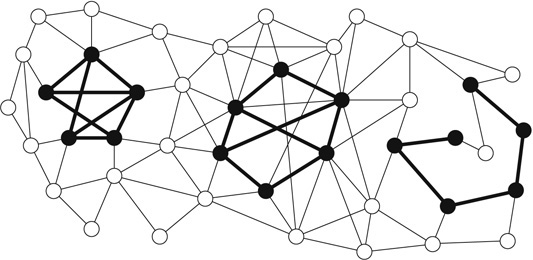
\includegraphics[width=1.5in]{images/good_cluster}
    \caption{\label{fig:comp_cluster} Drei verschiedene Cluster unterschiedlicher Qualität \cite{Schaeffer}}
  \end{figure}
  
  \subsection{k-Cliques}
  \label{sec:k_cliques}
  	Einen Teilgraphen $\Omega$ mit $k$ Knoten nennt man $k$-Clique, falls alle $k$ Knoten dieses 
  	Teilgraphen direkt miteinander verbunden sind, und $\Omega$ somit vollst"andig ist \cite{CPM}. 
  	Die entstehende Topologie des Teilgraphen $\Omega$ ist natürlich vom Parameter $k$ abh"anging.
  	Abb. \ref{fig:k_cliques} zeigt k-Cliques f"ur verschiedene Werte von $k$.
  	
  	\begin{figure}[h]
  	 \centering
  	 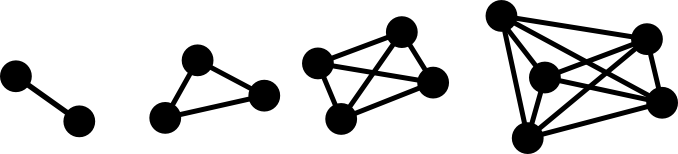
\includegraphics[width=2in]{images/k-cliques-example}
  	 \caption{\label{fig:k_cliques} Topologien f"ur k-Cliques mit k=2,3,4,5}
  	\end{figure}

  	
  	Da jede k-Clique vollst"andig ist, ist die in Kapitel \ref{sec:properties} definierte
  	interne Graphdichte mit $\rho_{int}(\Omega)=1$ maximal. Somit stellen k-Cliques theoretisch gute 
  	Kandidaten f"uer Cluster da. Beschr"ankt man sich bei der Clusterfindung auf einzelne k-Cliques,
  	werden in den meisten F"allen viele Cluster nicht gefunden, da Forderung an einen vollst"andig
  	verkn"upften Cluster zu restriktiv ist.
    
  \subsection{Dynamische Graphen}
	Ein klassicher Graph $\Omega=(V,E)$ ist eine Kombination einer Menge an Knoten $V$ und
	Kanten $E$ zu einem bestimmten Zeitpunkt $t$. F"ur viele Anwendungen
	ist es aber essentiell das Netzwerk "uber einen Zeitraum mit mehreren Zeitschritten $t_i$ zu
	betrachten und untersuchen.
	
	Das Konzept der \emph{dynamischen Graphen}\cite{modularity} stellt die zeitliche Ver"anderung eines Graphen
	als geordnete Folge von statischen Teilgraphen f"ur jeden Zeitpunkt $t=1,...,n$ da:
	\begin{align}
		\Upsilon=\{\Omega_1=(V_1, E_1), \Omega_2=(V_2, E_2), ..., \Omega_n=(V_n,E_n)\}
	\end{align}
	wobei $\Omega_i$ der Konfiguration des dynamischen Graphen $\Upsilon$ zum Zeitpunkt $i$ entspricht.
	Da alle $V_i, E_i$ f"ur alle Werte von $i$ unabh"angig sind, ist es m"ogich das zu jedem Zeitschritt
	sowohl Kanten als auch Knoten hinzugef"ugt oder verschwinden k"onnen.
  
\section{Clustering in statischen Graphen}
  \label{sec:static_clustering}

  Viele Clustering Verfahren f"ur dynamische Graphen basieren auf Verfahren zur Clusterung klassischer,
  statischer Graphen. Da dynamische Graphen aufgrund der Zeitanh"angigkeit weitere Komplexit"at einf"uhren,
  ist es sinnvoll als erstes diese Clusteringmethoden f"ur statische Graphen zu betrachten.
  In diesem Kapitel wird versucht die Vielzahl verschiedener Verfahren anhand ihrer grunds"atzlichen Eigenschaften
  in verschiedene Kategorien zu klassifizieren, sowie eine kurze Erkl"arung ihrer Funktionsweise zu geben.
  
  Nach Schaeffer \cite{Schaeffer} lassen sich Clustering Verfahren grunds"atzlich in lokale oder globale
  Verfahren einteilen. Hierbei werden die Verfahren entweder global auf den ganzen Graph angewendet,
  oder nur lokal auf einen Teilgraphen. Entsprechend ben"otigen globale Verfahren Informationen "ueber 
  die Topologie des gesammten Graphen, w"ahrend bei bei lokalen Verfahren nur rekursiv die Nachbarschaft
  eines einzelnen Knotens betrachtet wird, somit auch Netzwerke betrachtet werden k"onnen, die a priori
  nicht komplett bestimmt sind.
  
  Entsprechend bieten lokale Verfahren eine bessere Skalierbarkeit als Globale, falls das Clustering nur
  auf einen Teilgraphen angewendet werden soll, da die Topologie des restlichen Graphen nicht bekannt sein muss.
  Weiterhin haben diese Verfahren den Vorteil, dass das Clustering nur von der lokalen Struktur anh"angt und eine
  lokale "Anderung im Graphen auch nur das Clusterung in deren Umgebung beeinflusst. Deshalb eignen sich lokale
  Verfahren in Anwendungen, bei denen die Nachbarschaft einzelner Knoten schnell und h"aufig untersucht werden soll.
  
  
    \begin{table}[h]
    %% Table captions on top in journal version
    \caption{\label{tab:static_methods} Einteilung der Clusteringverfahren f"ur statische Graphen}
    \scriptsize
    \begin{center}
      \begin{tabular}{c|l|c}
	& Globale Verfahren & Lokale Verfahren\\
	\hline
	Top-Down  & Spektrale Methoden       & \\
	          & Random Walk Methoden     & \\
	          & Maximaler Fluss Methoden & \\
	\hline
	Bottom-Up & Modularit"atsoptimierung & CPM \\
	          & N"achste Nachbarn Methode & 
      \end{tabular}
    \end{center}
  \end{table}
  
  \subsubsection*{Globale Verfahren}
  Die Familie der globalen Verfahren l"asst sich noch mal in sogenannte \emph{Top-Down}, sowie
  \emph{Bottom-Up} Methoden \cite{Schaeffer} unterteilen. Bei Top-Down Verfahren wird der Graph rekursiv anhand
  verschiedener Kriterien in immer kleinere Methoden unterteilt, w"ahrend bei Bottom-Up Verfahren
  viele kleinere Cluster sukzessive zu gr"osseren zusammen gefasst werden, bis das Clustering einem
  Abbruchkriterium gen"ugt.
  
  Ein Vertreter der Top-Down Methoden, sind die sogenannten \emph{Spektralen Methoden}. Sie basieren auf den
  Eigenwerten und Vektoren der Laplace-Matrix des Graphen. Die Laplace Matrix eines Graph
  $\Omega=(V,E)$ ist definiert als
  \begin{align}
    L(\Omega)&=D(\Omega)-A(\Omega)
  \end{align}
  wobei $D(\Omega)=diag(\{d(v_1), ..., d(v_n)\})$ die Degreematrix von $\Omega$ ist \cite{graphcontrol}.
  $A(\Omega)$ ist die sogenannte Adjacency Matrix von $\Omega$, und definiert als
  \begin{align}
   \left[A\right]_{ij}&= \begin{cases}
			    1 & \text{falls zwischen }v_i\text{ und }v_j\text{ eine Kante besteht}\\
			    0 & \text{sonst}
			  \end{cases}
  \end{align}
  Da die Laplace Matrix eine symmetrische, positiv semidefinite Matrix ist \cite{graphcontrol}, sind alle Eigenwerte $\lambda_i \ge 0$
  und die korrespondierenden Eigenvektoren bilden ein orthogonales System. Ordnet man die Eigenwerte in
  aufsteigender Reihenfolge $\lambda_1 \le \lambda_2 \le \dots \le \lambda_n$, so folgt aus der positiv Semidefinitheit
  von L dass $\lambda_1 = 0$. Ist weiterhin $\lambda_2 > 0$ so existieren keine isolierten Teilgraphen im kompletten
  Graph[Buch]. Die Algorithmen der spektralen Clustering Methoden benutzen typischerweise die Komponenten des Fiedler
  Vektors -den Eigenvektor von $\lambda_2$- um die Knoten eins Graphen zu vergleichen und clustern \cite{Schaeffer}.

  Ein weitere Gruppe von Methoden die den Top-Down Ansatz verfolgen, sind die sogenannten \emph{Random Walk} oder
  \emph{Markov Ketten Methoden}. Diese Verfahren basieren auf einem zuf"alligen Weg $\xi$ fester L"ange durch den Graph.
  Dabei wird $\xi$, ausgehend von einem Startknoten $v_{start}$, iterativ "uber eine zuf"allige Auswahl
  der direkten Nachbarn des jeweils aktuellen Knoten aufgebaut. Aufgrund der h"oheren Dichte in Clustern, wird der Weg
  $\xi$ die Knoten des selben Clusters wie $v_{start}$ h"aufiger besuchen als Knoten ausserhalb des Clusters.
  Abb. \ref{fig:random_walk} zeigt einen Beispielgraph mit zwei Clustern. Wird ein Weg ausgehend von einem weisen
  Knoten aufgebaut, ist es f"ur einen zuf"alligen Weg nur auf einem Knoten m"oglich den linken Cluster zu verlassen,
  und somit werden die weisen Knoten des linken Clusters mit einer h"oheren Wahrscheinlichkeit besucht. 

    \begin{figure}[h]
    \centering
    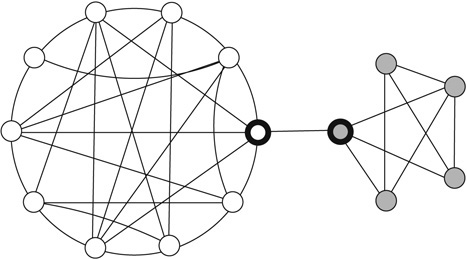
\includegraphics[width=2in]{images/random_walk}
    \caption{\label{fig:random_walk} Graph mit zwei Clustern. Beginnt man einen Random Walk bei einem Knoten des weisen Clusters
	      ist die Wahrscheinlichkeit im n"achsten Schritt einen weiteren weisen Knoten dieses Clusters zu erreichen h"oher,
	      als den Cluster zu verlassen \cite{Schaeffer}}
    \end{figure}
    
  F"ur gewichtete Graphen eignen sich auch die \emph{Maximaler Fluss Methoden} um ein Clustering duchzuf"uhren. Sie
  geh"oren ebenfalls zu der Gruppe der Top-Down Verfahren, und versuchen einen minimalen Schnitt \cite{Schaeffer} des Graphen zu finden. 
  Dazu werden Str"omungsberechnungen auf dem Graphen durchgef"uhrt, wobei ein Fluss zwischen zwei Knoten nur "uber eine Verbindungskante bestehen kann.
  Da aufgrund des \emph{Minimum cut, maximum Flow Theorms} der Schnitt eins Graphen beim maximalen Fluss am geringsten ist, l"asst sich dieser "uber
  den maximalen Fluss auf den Kanten des Graphen finden. Flake et al.\cite{flake} berechneten hierzu den Fluss mithilfe k"unstlich hinzugef"ugter
  Senken, und erzeugten daraus einen Minimum-cut Tree\cite{minimum_cut_tree} um das Clustering auf einem Graphen durchzuf"uhren.
  
  Beispiele f"ur Methoden, die einen Bottom-Up Ansatz werden sind unter anderem die \emph{Modularit"atsoptimierung} welche
  in Kaptiel \ref{sec:modularity} genauer behandelt wird. Eine weitere Vertreter ist die sogenannte \emph{N"achste Nachbarn Methode}\cite{Schaeffer}, welche
  h"aufig auch bei allgmeinen Klassifizierungsproblmen angewendet wird. Um die N"achste Nachbarn Methode auf Graphen anwenden
  zu k"onnen, muss eine "Ahnlichkeit zwischen zwei Knoten definiert werden. Eine solche "Ahnlichkeit
  kann z.B. anhand von vorhandenen Metadaten jedes Knoten erfolgen, oder anhand der Schnittmenge der direkten Nachbarn zweier
  Knoten. Im ersten Schritt wird f"uer jeden Knoten des Graphen derjenige Nachbar gesucht, f"uer welchen die "Ahnlichkeit am gr"ossten ist.
  Diese beiden Knoten bilden nun einen Cluster. In den darauffolgenden Schritten, werden nun die bereits gefunden Cluster auf "Ahnlichkeit
  untersucht, und zu gr"osseren Cluster zusammengef"ugt, bis das Clustering beendet ist.
  
  
  \subsection{Modularit"atsoptimierung}
    \label{sec:modularity}
    Das Verfahren der Modularit"atsoptimierung ist ein weiterer Vertreter der Bottom-Up Ans"atze. Es versucht eine Partitionierung
    des Graphen zu finden, f"ur die die Modularit"at maximal wird. Hierbei ist die Modularit"at ein Ma"s, in wie fern die gew"ahlte
    Partitionierung $C(\Omega)$ eines Graphen $\Omega$ einem guten Clustering entspricht. Gesucht ist somit eine optimale Partitionierung welche dem Clustering des Graphen entspricht.
    Mathematisch ist die Modularit"at $Q(C)$ definiert als \cite{modularity}:
    \begin{align}
      Q(C)=\frac{1}{2|E|}\sum\limits_{u,v \in V}\left[ A_{uv} - \frac {k_vk_u}{2|E|}\delta \left( c(u), c(v)\right) \right]
    \end{align}
    wobei $A_{uv}=1$ falls eine Kannte zwischen $u$ und $v$ existiert, ansonsten 0. $k_u = d(u)$ ist der Grad des Knoten, und
    $c(u)$ diejenige Partition die den Knoten $u$ enthält. Weiterhin ist $\delta \left(c(u),c(v)\right)$ falls $c(u)=c(v)$,
    ansonsten 0.
    Somit repräsentiert die Modularit"at die Summe aller Kanten innerhalb einer Partition minus der Anzahl der Kanten, falls diese 
    zuf"allig verteilt w"aren.
    
    Der trivialste Ansatz diejenige Partitionierung $C(\Omega)$ zu finden welche die Modularit"at maximiert, w"are die Berechnung
    aller m"oglichen Partitionen und ihrer dazugeh"origien Modularit"at. Es ist aber offensichtlich, dass bei steigender 
    Graphgr"osse die Anzahl m"oglicher Partitionen rasant steigt. Weiterhin wurde gezeigt \cite{modularity_nphard}, dass das Problem
    eine optimale Partition zu finden NP-Vollst"andig ist.
    
    Eine optimale Partitionierung, und somit ein Clustering kann mithilfe der Heuristik von Blondel et al. \cite{modularity_heuristic}
    approximiert werden. Der wesentliche Bestandteil
    der Heuristik ist die Tatsache, das die "Anderung der Modularit"at $\Delta Q$, falls ein Knoten $v_i$ in den Cluster $C$ verschoben
    wird, lokal effizient berechnet werden kann:
    \begin{align}
     \Delta Q &= \left[ \frac{\sum_{in}+k_{i,in}}{2m} - \left( \frac{\sum_{tot}+k_i}{2m} \right)^2 \right] -
     \left[ \frac{\sum_{in}}{2m} - \left( \frac{\sum_{tot}}{2m} \right)^2 - \left( \frac{k_i}{2m} \right)^2 \right]
    \end{align}
    wobei $\sum_{in}$ die Summe der Gewichte aller Kanten des Clusters $C$ ist, $\sum_{tot}$ die Summe der Gewichte aller Kanten welche
    mit Knoten des Cluster $C$ verbunden sind, $k_i$ ist die Summe der Gewichte aller Kanten des Knoten $v_i$, $k_{i,in}$ ist die
    Summe der Gewichte aller Kanten welche den Knoten $i$ mit Knoten aus $C$ verbinden, und $m$ die Anzahl aller Kanten im Graph.
    Hierbei bleibt zu erw"ahnen, das sogenannte \emph{Selfloops}, also Kanten von $v_i$ nach $v_i$ erlaubt sind, und sogar
    ein wesentlicher Teil der Heuristik darstellen.
    
    Die Heuristik l"auft nun wie folgt ab:
    \begin{enumerate}
      \item F"ur jeden Knoten wird ein einzelner Cluster erstellt, der nur diesen einen Knoten enth"alt
      \item Berechnung der $\Delta Q$ f"ur das Verschieben eines Knoten $v_i$ in die Cluster seiner 
      		direkten Nachbarn. Anschlie"send wird $v_i$ in den Cluster desjenigen Nachbarn $v_j$ verschoben,
      		dessen $\Delta Q$ am gr"ossten ist. Ist die Zunahme der Modularit"at f"ur jeden Nachbarn negativ,
      		so bleibt der Knoten $v_i$ in seinem Cluster. Dieser Schritt wird solange wiederholt, bis sich
      		ein lokales Maxima der Modularit"at einstellt. Dabei ist es durchaus m"oglich das ein Knoten
      		mehrmals betrachtet wird.
      \item Ist ein lokales Maxima erreicht, wird einer neuer Graph aufgebaut. Dabei entsprechen die bisherigen
      		Cluster den Knoten des neuen Graph. Diese sind verbunden falls mindestens eine Kante zwischen
      		je einem Knoten der beiden Cluster existiert und das Gewicht dieser Kante ist die Summer
      		der Gewichte aller Kanten zwischen diesen Clustern. Kanten innerhalb eines Cluster f"uhren zu einem
      		Selfloop dessen Gewicht die Summer der Gewichte dieser Kanten ist. 
      \item F"uhre Schritte 1-3 wiederum auf den neuen Graph aus, solange bis die Modularit"at nicht
      		weiter erh"oht werden kann.
    \end{enumerate}
    
  \subsection{Clique Percolation Method (CPM)}
    \label{sec:CPM}
    Alle bisher vorgestellten Methoden waren globale Clusteringverfahren. Ein lokales Verfahren ist die
    \emph{Clique Percolation Method (CPM)}\cite{CPM}, welche auf den in Kap. \ref{sec:k_cliques}
    vorgestellten k-Cliques beruht. Hierzu wird eine Nachbarschaftsbeziehung zwischen k-Cliques definiert, 
    bei der zwei k-Cliques benachbart sind, falls diese sich $k-1$ Knoten teilen. 
    
    Ein Cluster in der CPM ist definiert als eine maximale Menge von k-Cliques, welche "uber eine Nachbarschaft
    erreichbar sind. Dabei wird die CPM jeweils f"ur ein festgelegtes $k$ durchgef"uhrt. Es exisitieren 
    verschiedene Algorithmen mithilfe derer eine CPM durchgef"uhrt werden kann, z.B. der Bron-Kerbosch Algorithmus.
    
    Abb. \ref{fig:CPM} zeigt die gefundenen 3-Cliques Cluster einer CPM f"ur einen willk"urlichen Graphen.
    Im linken sowie rechten Graph werden jeweils zwei Cluster gefunden, welche durch graue und schwarze
    Einf"arbung hervorgehobenen sind. Im rechten Graph ist zu erkennen, dass sich Cluster, welche mithilfe einer
    CPM gefunden wurden, ein oder mehrere Knoten teilen k"onnen. Somit ist es auch m"oglich "uberlappende Cluster
    in einem Netzwerk zu finden, welche vor allem in sozialen Netzwerken auftreten.
    \begin{figure}[h]
     \centering
     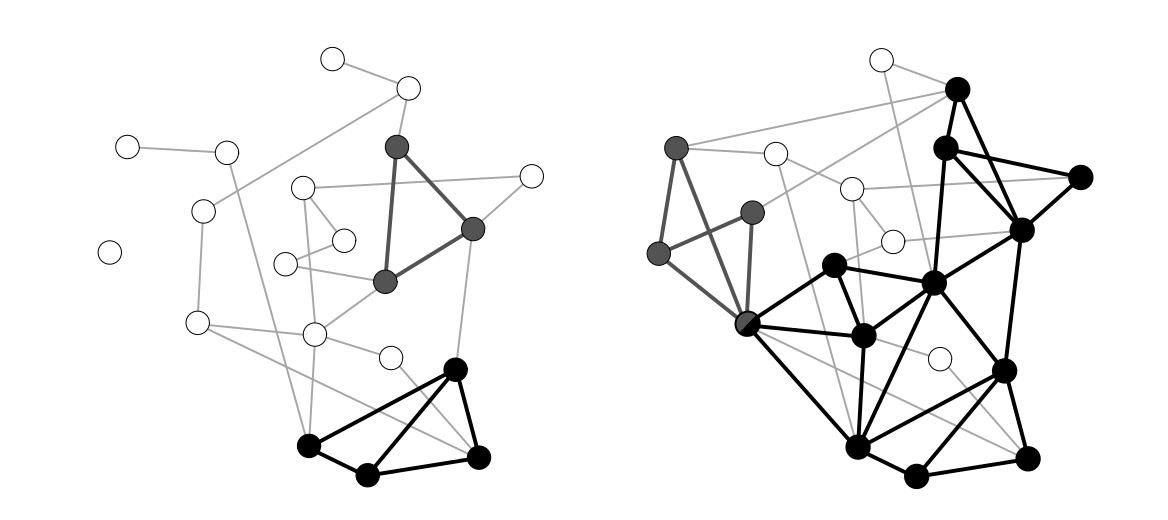
\includegraphics[width=2.5in]{images/k-cliques}
     \caption{\label{fig:CPM} Gefundene 3-Clique Cluster zweier zuf"alliger Graphen. In beiden Graphen werden jeweils zwei
		Cluster gefunden, welche schwarz und grau hervorgehoben sind \cite{CPM}}
    \end{figure}


\section{Clustering in dynamischen Graphen}
  \label{sec:dynamic_clustering}
  Bei einem Clustering eines dynamischen Graphens, ist neben der Identifikation der Cluster ansich, auch deren
  zeitlichen Verlauf von Interesse. Hierzu k"onnen die bisher vorgestellten Clusteringverfahren f"ur statische
  Graphen erweitert oder modifiziert werden, damit die gefundenen Cluster "ueber die Zeitschritte verfolgt werden
  k"onnen.
  
  Hierzu lassen sich die Verfahren in zwei Klassen einteilen. \emph{Evolution"are Clustering Verfahren}\cite{evolutionary_clustering}
  verwenden Graphinformationen mehrerer konsekutiver Zeitschritte um ein Clustering durchzuf"uhren. Zum Beispiel verwendet die Erweiterung der CPM
  in Kap. \ref{sec:CPM_time} Graphinformationen des aktuellen, sowie des n"achsten Zeitschritt. Ziel der evolution"aren Clusteringverfahren
  ist es ein "uber mehrere Zeitschritte konsistentes Clustering zu finden, in welchem weiche "Uberg"ange zwischen Clustern der einzelnen Zeitschritten
  besteht.
  
  Die andere Klasse der Clusteringverfahren dynamischer Graphen wird hier \emph{Time-step Clustering} genannt. Im Gegensatz zu den evolution"aren
  Clusteringverfahren, wird ein Clusteringverfahren separat auf den statischen Graph jedes einzelnen Zeitschritts angewendet. Dies hat den Vorteil das
  Clusteringverfahren statischer Graphen, somit auch die in Kap. \ref{sec:static_clustering} vorgestellten Verfahren, ohne Modifikation
  verwendet werden k"onnen. Da nur die Informationen des aktuellen Zeitschritt verwendet werden, dass sich die gefunden Cluster in konsekutiven
  Zeitschritten sehr stark "andern.
  
  F"ur Verfahren beider Klassen ist es notwendig gefundene Cluster verschiedener Zeitschritte zu vergleichen, um spezifische Cluster "uber
  mehrerer Zeitschritte verfolgen zu k"onnen. Dazu kann der \emph{Jaccard-Koeffizient} verwendet werden, mithilfe dessen zwei Mengen auf "Ahnlichkeit
  untersucht werden k"onnen. F"ur die Mengen $A$ und $B$ ist er definiert als \cite{timestep}:
  \begin{align}
    J(A,B)=\frac{|A \cap B|}{|A \cup B|}
  \end{align}
  wobei $|A|$ die Anzahl der Elemente in $A$ ist. Somit ist der Wertebereich des Jaccard-Koeffizient $[0,1]$ mit 1 als maximaler "Ubereinstimmung.
  
  \subsection{Evolution eins Clusters}
    \label{sec:evolution}
    Betrachtet man den zeitlichen Verlauf eines Clusters, so k"onnen verschiedene Ereignisse auftreten. Zu jedem Zeitpunkt kann ein neuer Cluster
    entstehen, ebenso kann sich ein bestehender Cluster aufl"osen. Weiterhin k"onnen neue Cluster entstehen, falls sich bisherige grosse Cluster
    teilen. Ebenso ist das Gegenteil m"oglich, und mehrere kleinere Cluster formieren sich im n"achsten Zeitschritt zu einem Grossen.
    Im einfachsten Fall bleib ein Cluster im n"achsten Zeitschritt konstant, w"achst oder schrumpft indem neue Knoten hinzukommen oder weggehen.
    In Abb. \ref{fig:evolution} sind alle m"oglichen Ereignisse noch einmal dargestellt.
    \begin{figure*}[t]
      \centering
      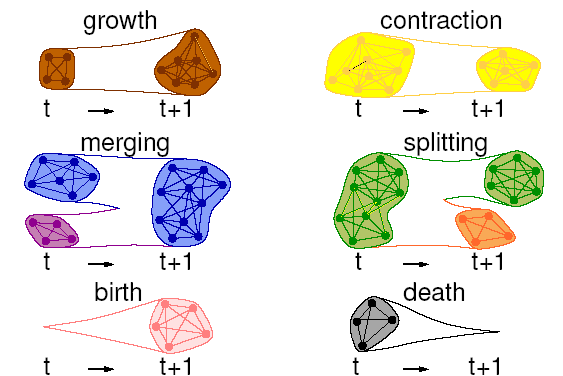
\includegraphics[width=11cm]{images/evolution_alone}
      \caption{M"ogliche Ereignisse im zeitlichen Verlauf eines Clusters \cite{CPM_time}}
      \label{fig:evolution}
    \end{figure*}
  \subsection{Erweiterung der CPM}
    \label{sec:CPM_time}
    Palla et al. haben in \cite{CPM_time} die in Kaptiel \ref{sec:CPM} vorgestellte Clique Percolation Method erweitert, um sie auf dynamische
    Graphen anzuwenden. Dabei wird ein evolution"arer Ansatz verwendet, welcher den Graphen $\Omega_{t}$ zum Zeitpunkt $t$, als auch $\Omega_{t+1}$
    benutzt.
    
    Im ersten Schritt wird mithilfe der CPM f"ur statische Graphen jeweils ein Clustering f"ur $\Omega_{t}$ und $\Omega_{t+1}$ durchgef"uhrt.
    Anschlie"send wird ein Verbundgraph $\Omega_{t,t+1} = \Omega_{t} \cup \Omega_{t+1}$ konstruiert, welcher alle Knoten und Kanten aus
    $\Omega_t$ und $\Omega_{t+1}$ enth"alt. Auf diesen Verbundgraph wird wiederum eine CPM angewendet. Da bei der Vereinigung zweier Graphen
    keine Kanten oder Knoten entfernt werden, existiert f"ur jeden Cluster in $\Omega_t$ und $\Omega_{t+1}$ genau ein Cluster in $\Omega_{t,t+1}$.
    Enth"alt ein Cluster im Verbundgraph jeweils einen einzelnen Cluster aus $\Omega_t$ und einen einzelnen Cluster aus $\Omega_{t+1}$,
    so k"onnen diese identifiziert werden. Falls ein Cluster des Verbundsgraph mehrere Cluster der aus $\Omega_t$ oder $\Omega_{t+1}$
    enth"alt, werden die Cluster anhand des relativen Knoten "Uberlapps identifiziert. Details des Verfahren in \cite{CPM_time}.
    
    In Abb. \ref{fig:CPM_time} werden die einzelnen Schritte der CPM Erweiterung graphisch dargestellt. Der Graph zum Zeitpunkt $t$ wird
    in blau dargestellt, der Graph zum Zeitpunkt $t+1$ in gelb. Die Kreise zeigen die jeweils gefundenen Cluster an. Der Verbundgraph ist
    in der Mitte dargestellt. Gr"un gef"arbte Knoten und Kanten sind dabei in beiden Zeitschritten vorhanden, blau und gelbe nur in den
    Zeitschritten entsprechender Farbe.
    
    \begin{figure}[h]
      \centering
      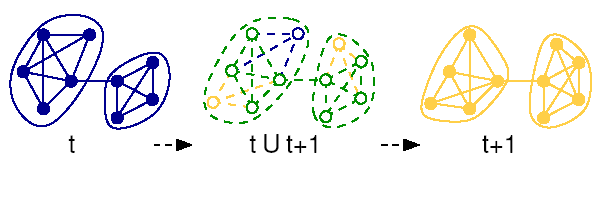
\includegraphics[width=3in]{images/CPM_time}
      \caption{\label{fig:CPM_time} Zwei Zeitschritte eines dynamischen Graphen. Der mittlere Graph ist die Vereinigung der Graphen beider Zeitschritte \cite{CPM_time}}
    \end{figure}

    
  \subsection{Dynamic Communities}
    Ein wichtiger Teil eines Time-Step Clusteringverfahrens ist neben dem eigentlichen Clustering, das Identifizieren gleicher Cluster
    "uber mehrere Zeitschritte. Hierzu haben Greene et al. in \cite{timestep} ein generelles Framework vorgestellt, welches auf den
    in Kap. \ref{sec:evolution} gezeigten Ereignissen basiert. Da es weiterhin unabh"angig vom verwendeten Clustering Verfahren ist,
    l"asst es sich mit allen in Kap. \ref{sec:static_clustering} vorgestellten Verfahren kombinieren.
    
    Betrachtet man einen dynamischen Graphen $\Upsilon = \{ \Omega_1, \dots, \Omega_n \}$ als eine geordnete Folgen statischer
    Graphen $\Omega_t$ zum Zeitpunkt $t$ und wendet ein Time-Step Clustering an, erh"ahlt man ein Clustering
    $\mathbb{C}_t = \{ C_{t,1}, \dots, C_{t,k}\}$ f"ur jeden einzelnen Zeitschritt.
    
    Ein Kernkonzept des in \cite{timestep} vorgestellten Verfahrens sind sogenannte \emph{Dynamic Communities}. Diese Dynamic
    Communities $D_i$ repräsentieren den zeitlichen Verlauf eines einzelnen Cluster $C_i$ im Graph. Sie lassen sich als eine zeitlich 
    geordnete Folge $D_i = \{ C_{1,i}, \dots, C_{n,i} \}$ einzelner Konfigurationen des Clusters $C_i$ zu unterschiedlichen Zeitpunkten
    darstellen. Abb. \ref{fig:dynamic1} zeigt den Verlauf dreier Dynamic Communities "uber drei Zeitschritte. Es ist an $D_3$ ersichtlich das
    nicht f"uer alle Zeitschritte eine Konfiguration $C_{t,i}$ vorhanden sein muss. Die zeitlich letzte bekannte Konfiguration
    einer Dynamic Community wird die Front $F_i$ genannt, welche f"ur verschiedene $D_i$ nicht unbedingt zum selben Zeitpunkt sein muss.
    \begin{figure}[h]
      \centering
      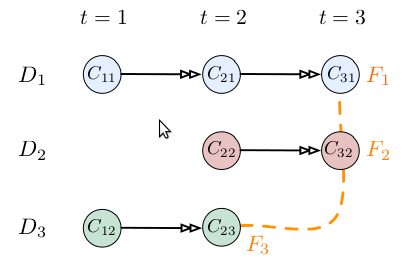
\includegraphics[width=2.5in]{images/dynamic_communities1}
      \caption{\label{fig:dynamic1} Drei Dynamic Communities "uber drei Zeitschritte, bei denen Geburt und Todesereignisse auftreten.\cite{timestep}}
    \end{figure}
    
    Die Dynamic Communities in Abb \ref{fig:dynamic1} sind:
    \begin{itemize}
      \item $D_1 =\{C_{1,1}, C_{2,1}, C_{3,1}\}$
      \item $D_2 =\{C_{2,2}, C_{3,2}\}$
      \item $D_3 =\{C_{1,2}, C_{2,3}\}$
    \end{itemize}
    
    F"ur jeden Zeitschritt $t$ werden die gefundenen Cluster $C_i$ des Clustering $\mathbb{C}_t$ mit den Fronten der Dynamic Communities
    verglichen um gleiche Cluster in konsekutiven Zeitschritten zu finden. Hierzu wird der in Kap. \ref{sec:dynamic_clustering}
    vorgestellte Jaccard-Koeffizient verwendet. Dabei sind die
    Front $F_j$ und der Cluster $C_{t,i}$ gleich falls $J(F_j,C_{t,i})$ gro"ser einem bestimmten Wert $\theta$ ist. Da in dynamischen Graphen
    die in Kap. \ref{sec:evolution} beschriebenen Ereignisse auftreten k"onnen, ist es durchaus m"oglich, dass ein Cluster $C_{t,i}$ des
    Clustering $\mathbb{C}_t$ keiner, einer oder mehreren Fronten zugeordnet werden kann. Dabei gelten folgende Regeln f"ur die 
    einzelnen Ereignisse im zeitlichen Verlauf eines Clusters:
    \begin{itemize}
      \item \textbf{Geburt:} \hfill \\
	    Falls ein Cluster $C_{t,i}$ zum Zeitpunkt $t$ keiner bisherigen Front zugeordnet werden kann, wird eine neue Dynamic Community
	    $D_i$ angelegt, welche $C_{t,i}$ enth"alt. Die Dynamic Community $D_2$ in Abb. \ref{fig:dynamic1} wird zum Zeitpunkt $t=2$ geboren. 
      \item \textbf{Tod:} \hfill \\
	    Eine bestehende Dynamic Community $D_i$ kann sich auch zu jedem Zeitschritt auch aufl"osen. Dies ist der Fall, falls in $d$ konsekutiven
	    Zeitschritten kein Cluster finden l"asst, der der Front $F_i$ entspricht. Nach dem Tod von $D_i$ werden die gefunden Cluster nicht mehr mit
	    $F_i$ verglichen. Ist $d>1$ so kann eine Dynamic Community mehrere Zeitschritte ohne einen entsprechenden Cluster des aktuellen Zeitschritts bestehen.
	    Ein Beispiel f"ur den Tod einer Dynamic Community ist $D_3$ in Abb. \ref{fig:dynamic1}, falls f"ur $t>3$ keine Cluster gefunden werden welche $F_3$ entsprechen.
      \item \textbf{Zusammenschluss:} \hfill \\
	    Zwei Dynamic Communities fallen zusammen, falls ein Cluster $C_{t,m}$ zwei Fronten $F_i$ und $F_j$ zugeordnet werden kann. Beiden Dynamic Communities
	    $D_i$ und $D_j$ wird der Cluster $C_{t,m}$ hinzugef"ugt. Ein Beispiel hierf"ur sind $D_1$ und $D_2$ in Abb. \ref{fig:dynamic2}.
      \item \textbf{Trennung:} \hfill \\
	    Lassen sich zwei Cluster $C_{t,i}$ und $C_{t,j}$ der gleichen Front $F_m$ zuordnen, so teilt sich die Dynamic Community im aktuellen Zeitschritt.
	    Dabei wird $D_m$ einer der beiden Cluster $C_{i,t}$ oder $C_{j,t}$ hinzugef"ugt, und eine neue Dynamic Community $D_l$ angelegt, welche die bisherigen
	    Elemente von $D_m$ enth"alt, zus"atzlich des anderen Clusters.
	    Ein Beispiel sind die Dynamic Communities $D_3$ und $D_4$ in Abb. \ref{fig:dynamic2}.
    \end{itemize}
    Somit sind die Dynamic Communities in Abb. \ref{fig:dynamic2}:
    \begin{itemize}
      \item $D_1 =\{C_{1,1}, C_{2,1}, C_{3,1}\}$
      \item $D_2 =\{C_{1,2}, C_{2,1}, C_{3,1}\}$
      \item $D_3 =\{C_{1,3}, C_{2,2}, C_{3,2}\}$
      \item $D_4 =\{C_{1,3},C_{2,3}, C_{3,3}\}$
    \end{itemize}

    
    \begin{figure}[b]
      \centering
      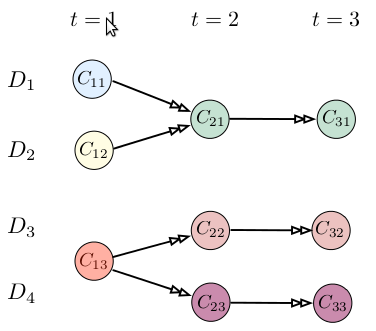
\includegraphics[width=2.5in]{images/dynamic_communities2}
      \caption{\label{fig:dynamic2}  Drei Dynamic Communities, bei denen ein Zusammenschluss und Trennungsereigniss auftritt \cite{timestep}}
    \end{figure}
    Folgende Schritte werden somit im \cite{timestep} vorgestellten Algorithmus durchgef"uhrt:
    \begin{enumerate}
      \item Anwenden eines Clusteringverfahren auf den statischen Teilgraphen $\Omega_0$ zum Zeitpunkt $t=0$ des dynamischen Graphen $\Upsilon$. F"ur jeden gefundenen
	    Cluster wird eine Dynamic Community angelegt, welche diesen Cluster enth"alt.
      \item F"uhre ein Clustering des nachfolgenden Zeitschritt aus, um Menge der Cluster $\mathbb{C}_t$ zu erhalten.
      \item Wende auf jeden Cluster $C_{i,t} \in \mathbb{C}_t$ folgende Schritte an:
      \begin{enumerate}
	\item Finde alle Dynamic Communities $D_j$, f"ur die $J(C_{i,t},F_j) > \theta$ ist.
	\item Falls es keine solche Dynamic Community gibt, lege eine neue an welche $C_{i,t}$ enth"ahlt.
	\item Falls Dynamic Communities gefunden wurden, f"uge Jeder $C_{i,t}$ hinzu.
      \end{enumerate}
      \item Falls einer bestehenden Dynamic Community $D_i$ mehere Cluster zugeordnet wurden, wird f"ur jeden zus"atzlichen Cluster eine Kopie von $D_i$ erstellte,
	    welcher jeweils der jeweilige Cluster hinzugef"ugt wurde.
	    Anschlie"send werden die Fronten $F_i$ aller aktiven Communties auf den letzten bekannten Cluster aktualisiert.
      \item Wiederhole ab Schritt 2 bis alle Zeitschritte verarbeitet wurden.
    \end{enumerate}
    Hierbei entspricht der Schritt 3. (b) der Geburt einer neuen Community, der Schritt 3. (c) einem Zusammenschluss mehrere Communities falls Anzahl der "ubereinstimmenden
    Fronten $>1$ ist. In Schritt 4. wird der Fall behandelt, falls sich eine bestehende Dynamic Community in mehrere aufteilt.

\section{Fazit}
  In diesem Artikel wurde eine "Ubersicht verschiedenster Graphclustering Verfahren gegeben. Das Forschungsgebiet des Clustering statischer Graphen ist sehr gut
  erforscht, was die Vielzahl der vorgestellten Verfahren best"atigt. Hierbei stellen die Verfahren aus Kap. \ref{sec:static_clustering} nur eine sehr grobe "Ubersicht
  dar, da oftmals Variationen und zus"atzliche Heuristiken bestehen. Eine detaillierte Beschreibung, sowie weiterf"uhrende Literatur ist in \cite{Schaeffer} gegeben.
  In den letzten Jahren hat sich der Fokus der Forschung auf diesem Gebiet in Richtung dynamischer Graphen verschoben. Zwar ist es mit dem in \cite{timestep} vorgestellten
  Framework m"ogliche, jedes statische Clustering Verfahren auch f"ur dynamische Graphen anzuwenden, allerdings haben Time-Step Verfahren den Nachteil, dass gefunden Cluster
  durchaus "uber mehrere Zeitschritte sehr stark schwanken k"onnen.
  
  Pers"onlich sehe ich das gr"o"ste Potential in lokalen Verfahren wie der CPM. Diese bieten den Vorteil das der komplette Graph a priori nicht vorhanden sein muss, 
  dass das Clustering au"sschlie"slich auf bestimmte Bereiche angewendet werden kann und das bei lokalen "Anderungen nicht das komplette Clustering neu berechnet werden muss.
  Zwar ist die CPM aufgrund der maximalen Graphdichte der k-Cliques sehr restriktiv, allerdings existieren weitere Ideen, welche aus gefunden k-Cliques, sowie dem
  relativen Knoten"uberlapp benachbarter k-Cliques einen gewichteten Clique-Graph\cite{clique_graph} aufbauen, und somit neue M"oglichkeiten zur Clusterung bieten.
    
\bibliographystyle{abbrv}
%% use following if all content of bibtex file should be shown
% \nocite{*}
\bibliography{literatur}
\end{document}
